

\tikzset{every picture/.style={line width=0.75pt}} %set default line width to 0.75pt        

\begin{tikzpicture}[x=0.75pt,y=0.75pt,yscale=-1,xscale=1,scale=0.6, every node/.style={scale=0.6}]
%uncomment if require: \path (0,293); %set diagram left start at 0, and has height of 293

%Image [id:dp5236848150513451] 

\draw (136.7,134.11) node  {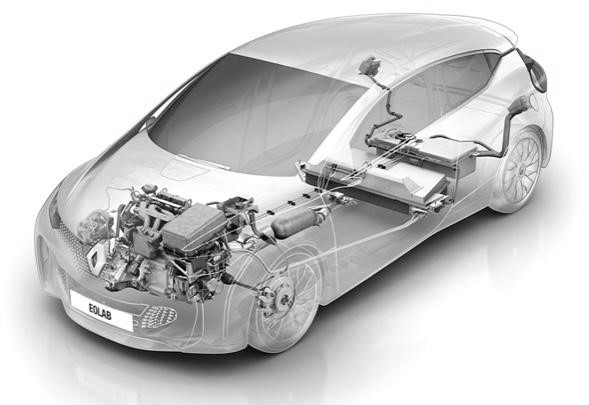
\includegraphics[width=204.75pt,height=138pt]{assets/cars.jpg}};
%Shape: Ellipse [id:dp22575039289402277] 
\draw  [color={rgb, 255:red, 255; green, 255; blue, 255 }  ,draw opacity=1 ][fill={rgb, 255:red, 255; green, 255; blue, 255 }  ,fill opacity=1 ] (11.33,122.73) .. controls (11.33,114.82) and (17.45,108.4) .. (25,108.4) .. controls (32.55,108.4) and (38.67,114.82) .. (38.67,122.73) .. controls (38.67,130.65) and (32.55,137.07) .. (25,137.07) .. controls (17.45,137.07) and (11.33,130.65) .. (11.33,122.73) -- cycle ;
%Shape: Ellipse [id:dp3623945699685074] 
\draw  [color={rgb, 255:red, 255; green, 255; blue, 255 }  ,draw opacity=1 ][fill={rgb, 255:red, 255; green, 255; blue, 255 }  ,fill opacity=1 ] (84.67,185.4) .. controls (84.67,177.48) and (90.79,171.07) .. (98.33,171.07) .. controls (105.88,171.07) and (112,177.48) .. (112,185.4) .. controls (112,193.32) and (105.88,199.73) .. (98.33,199.73) .. controls (90.79,199.73) and (84.67,193.32) .. (84.67,185.4) -- cycle ;
%Shape: Ellipse [id:dp8906821910938405] 
\draw  [color={rgb, 255:red, 255; green, 255; blue, 255 }  ,draw opacity=1 ][fill={rgb, 255:red, 255; green, 255; blue, 255 }  ,fill opacity=1 ] (207.33,53.4) .. controls (207.33,45.48) and (213.45,39.07) .. (221,39.07) .. controls (228.55,39.07) and (234.67,45.48) .. (234.67,53.4) .. controls (234.67,61.32) and (228.55,67.73) .. (221,67.73) .. controls (213.45,67.73) and (207.33,61.32) .. (207.33,53.4) -- cycle ;
%Shape: Ellipse [id:dp1843235766479494] 
\draw  [color={rgb, 255:red, 255; green, 255; blue, 255 }  ,draw opacity=1 ][fill={rgb, 255:red, 255; green, 255; blue, 255 }  ,fill opacity=1 ] (240.33,98.07) .. controls (240.33,90.15) and (246.45,83.73) .. (254,83.73) .. controls (261.55,83.73) and (267.67,90.15) .. (267.67,98.07) .. controls (267.67,105.98) and (261.55,112.4) .. (254,112.4) .. controls (246.45,112.4) and (240.33,105.98) .. (240.33,98.07) -- cycle ;
%Shape: Polygon Curved [id:ds2694891835945543] 
\draw  [draw opacity=0][fill={rgb, 255:red, 74; green, 145; blue, 158 }  ,fill opacity=0.25 ] (22.67,101.33) .. controls (32.67,96) and (57.33,94) .. (51.33,112) .. controls (45.33,130) and (50,119.33) .. (44,131.33) .. controls (38,143.33) and (27.33,164.67) .. (7.33,134.67) .. controls (-12.67,104.67) and (12.67,106.67) .. (22.67,101.33) -- cycle ;

%Shape: Polygon Curved [id:ds6576330285171925] 
\draw  [draw opacity=0][fill={rgb, 255:red, 139; green, 87; blue, 42 }  ,fill opacity=0.2 ] (96.67,166) .. controls (126.67,164.8) and (125.33,174.53) .. (119.33,192.53) .. controls (113.33,210.53) and (102,209.87) .. (94,210.53) .. controls (86,211.2) and (58.67,181.73) .. (67.33,177.87) .. controls (76,174) and (66.67,167.2) .. (96.67,166) -- cycle ;

%Shape: Polygon Curved [id:ds2775692663684084] 
\draw  [draw opacity=0][fill={rgb, 255:red, 206; green, 106; blue, 107 }  ,fill opacity=0.2 ] (248.33,75) .. controls (258.33,69.67) and (283,67.67) .. (277,85.67) .. controls (271,103.67) and (275.67,93) .. (269.67,105) .. controls (263.67,117) and (253,138.33) .. (233,108.33) .. controls (213,78.33) and (238.33,80.33) .. (248.33,75) -- cycle ;

%Shape: Polygon Curved [id:ds12005288403924697] 
\draw  [draw opacity=0][fill={rgb, 255:red, 245; green, 166; blue, 35 }  ,fill opacity=0.2 ] (138.4,48.87) .. controls (148.4,43.53) and (173.07,41.53) .. (167.07,59.53) .. controls (161.07,77.53) and (165.73,66.87) .. (159.73,78.87) .. controls (153.73,90.87) and (143.07,112.2) .. (123.07,82.2) .. controls (103.07,52.2) and (128.4,54.2) .. (138.4,48.87) -- cycle ;

%Shape: Polygon Curved [id:ds34961065781940404] 
\draw  [draw opacity=0][fill={rgb, 255:red, 190; green, 211; blue, 195 }  ,fill opacity=0.2 ] (217.07,33.2) .. controls (227.07,27.87) and (251.73,25.87) .. (245.73,43.87) .. controls (239.73,61.87) and (244.4,51.2) .. (238.4,63.2) .. controls (232.4,75.2) and (221.73,96.53) .. (201.73,66.53) .. controls (181.73,36.53) and (207.07,38.53) .. (217.07,33.2) -- cycle ;

%Shape: Ellipse [id:dp6562955430613056] 
\draw  [color={rgb, 255:red, 255; green, 255; blue, 255 }  ,draw opacity=1 ][fill={rgb, 255:red, 255; green, 255; blue, 255 }  ,fill opacity=1 ] (128.67,70.07) .. controls (128.67,62.15) and (134.79,55.73) .. (142.33,55.73) .. controls (149.88,55.73) and (156,62.15) .. (156,70.07) .. controls (156,77.98) and (149.88,84.4) .. (142.33,84.4) .. controls (134.79,84.4) and (128.67,77.98) .. (128.67,70.07) -- cycle ;

% Text Node
\draw  [draw opacity=0][fill={rgb, 255:red, 190; green, 211; blue, 195 }  ,fill opacity=0.2 ]  (222.07, 54.2) circle [x radius= 16.97, y radius= 15.56]   ;
\draw (211.07,45.6) node [anchor=north west][inner sep=0.75pt]    {$X^{2}$};
% Text Node
\draw  [draw opacity=0][fill={rgb, 255:red, 245; green, 166; blue, 35 }  ,fill opacity=0.2 ]  (143.4, 69.87) circle [x radius= 16.97, y radius= 15.56]   ;
\draw (132.4,61.27) node [anchor=north west][inner sep=0.75pt]    {$X^{3}$};
% Text Node
\draw  [draw opacity=0][fill={rgb, 255:red, 206; green, 106; blue, 107 }  ,fill opacity=0.2 ]  (253.33, 96) circle [x radius= 16.97, y radius= 15.56]   ;
\draw (242.33,87.4) node [anchor=north west][inner sep=0.75pt]    {$X^{4}$};
% Text Node
\draw  [draw opacity=0][fill={rgb, 255:red, 74; green, 145; blue, 158 }  ,fill opacity=0.35 ]  (27.67, 122.33) circle [x radius= 16.97, y radius= 15.56]   ;
\draw (16.67,113.73) node [anchor=north west][inner sep=0.75pt]    {$X^{1}$};
% Text Node
\draw  [draw opacity=0][fill={rgb, 255:red, 139; green, 87; blue, 42 }  ,fill opacity=0.2 ]  (100.33, 185) circle [x radius= 16.97, y radius= 15.56]   ;
\draw (89.33,176.4) node [anchor=north west][inner sep=0.75pt]    {$X^{5}$};


\end{tikzpicture}
